\documentclass[11pt]{article}

% ---- packages ----
\usepackage[utf8]{inputenc}
\usepackage[T1]{fontenc}
\usepackage[margin=1in]{geometry}
\usepackage{amsmath,amssymb}
\usepackage{booktabs}
\usepackage{graphicx}
\usepackage{microtype}
\usepackage{caption}
\usepackage[hidelinks]{hyperref}

\graphicspath{{figures/}}

% absorb minor justified-line slack so nothing bleeds into the margin
\emergencystretch=1em

% ---- title ----
\title{Ablating Persistent Structured State Collapses a Weak-Model
Scaffolding Harness: A Seed-Matched Component Study%
\thanks{All quantitative results regenerate from the archived databases and
scripts in the accompanying reproducibility package (Appendix~A).}}

\author{[Author name --- fill in]\\ \texttt{[affiliation / contact --- fill in]}}
\date{}

\begin{document}
\maketitle

\begin{abstract}
We study whether a scaffolding harness built around persistent structured
state can move a weak 4B language model from universal failure to majority
success on a 200-day business-operations simulator, and we test which
high-level harness treatment is necessary for the observed performance. Using a
simulator with deterministic transition dynamics, matched environment seeds,
and Vending-Bench economics [1] (supplier roster including adversarial
profiles), we compare three arms on \texttt{gemma3:4b}: a naive one-call-per-day
model baseline (\textbf{bare}), a deterministic scripted policy with no model
judgment (\textbf{scripts}), and the full harness combining persistent
structured state, financial gates, and specialized model seats
(\textbf{full}). Over $N=100$ matched seeds, bare fails 100\% of runs (median
net worth \$83), scripts fails 59\% (\$29), and full fails 46\% (\$1,415).
Paired comparisons strongly favor full over both baselines on net worth
(full$-$scripts $+$\$990/seed, Wilcoxon $p=1.3\times10^{-9}$). Decomposing
``failure,'' we find little evidence of a bankruptcy reduction versus the
scripted policy (44\% vs 47\%; paired risk difference $-3$~pp, 95\% CI
$[-11,+5]$); instead the harness's advantage grows with the success threshold,
from 3~pp at bankruptcy to 32~pp at a \$2,000 bar. A component ablation is
strongly asymmetric: removing the gate suite does not measurably degrade median
net worth or failure rate (paired median $\Delta=\$0$, composite-failure risk
difference $-1$~pp $[-11,+9]$), while removing persistent structured state
collapses performance to 100\% failure and a median net worth \emph{below} the
naive baseline. The removal-of-state arm retains the full call structure and
budget, ruling out decision budget or task decomposition \emph{alone} as
sufficient explanations. A seat-level ablation identifies pricing as a
necessary model-mediated contributor: replacing only the pricing seat with a
script erases the full arm's advantage --- the result is statistically
indistinguishable from scripts on composite failure and modestly \emph{worse}
on mean net worth ($N=100$). Consistent with this, among co-surviving runs the
full harness realizes substantially higher selling prices with no evidence of
increased sales volume. We interpret the state result as the harness supplying
persistent structured state the weak model cannot hold in-context; whether the
mechanism is persistence, denoised representation, or both is not separated
here. We report exploratory capability-gradient, live-adversary, and durability
studies in an appendix, and discuss threats to validity --- including the
inferential estimand, seed-holdout, decoding stochasticity, that the gates are
lightly stressed by this workload, and that we did not test a tool-enabled
model permitted to construct its own scaffold.
\end{abstract}

\section{Introduction}

Long-horizon agentic tasks --- where a model must act coherently across
hundreds of steps --- are a known weak point for language models, and a common
way to measure the weakness is to run a model ``bare'': a prompt, a tool
interface, and no persistent scaffolding. We argue this measures the absence of
scaffolding as much as the ceiling of the model, and we test what a scaffolding
harness contributes and \emph{which part of it} contributes. Throughout, we
scope claims to what a seed-matched ablation can support: components that are
\emph{necessary} for the observed performance under this workload, not general
laws about what agents need.

\paragraph{Contributions.}
\begin{enumerate}
\item A seed-matched three-arm comparison (naive baseline / scripted policy /
full harness) on a 200-day business simulator with adversarial supplier
profiles, $N=100$ (\S5.1).
\item A decomposition of ``failure'' into bankruptcy versus quality-of-survival
--- reported with paired risk differences and confidence intervals, and a full
seed-level transition table --- showing the harness's advantage grows with the
success threshold (\S5.2).
\item A behavioral analysis among co-surviving runs showing similar
late-horizon sales volume but a substantially higher realized selling price
under the full harness (\S5.3).
\item A component ablation with a strongly asymmetric result --- persistent
structured state is necessary for the observed performance; the financial gates
are not necessary for median performance or failure reduction under this
workload --- with decision budget and task decomposition controlled between the
full and no-state arms (\S5.4).
\item A seat-level ablation identifying pricing as a necessary model-mediated
contributor to the full harness's advantage (\S5.4).
\end{enumerate}

\paragraph{Research questions.}
\begin{itemize}
\item \textbf{RQ1.} Does a persistent-structured-state harness move a weak 4B
model from failure to majority success on this long-horizon task, relative to a
naive model baseline and a model-free scripted policy?
\item \textbf{RQ2.} Is the harness's advantage over the scripted policy
attributable to the model's judgment, and through what behavioral channel?
\item \textbf{RQ3.} Which harness component --- persistent structured state or
financial gates --- is necessary for the observed performance?
\item \textbf{RQ4.} Does the harness reduce outright failure (bankruptcy), or
improve the quality of surviving businesses?
\end{itemize}

\section{Related Work}

\paragraph{Long-horizon agent benchmarks.} Our economics (a \$500 starting
balance, a \$2/day operating fee, and bankruptcy after 10 consecutive unpaid
days) follow Vending-Bench [1], a benchmark designed to stress long-horizon
coherence rather than single-step reasoning; Vending-Bench itself reports that
leading models lose coherence over long runs. A broader line of agent
benchmarks --- GAIA [5] for general assistant tasks and $\tau$-bench [6] for
tool-and-policy-following in dynamic environments --- likewise finds that
headline capability degrades sharply once tasks require sustained, multi-step
execution rather than single-shot reasoning. We contribute a controlled
decomposition of \emph{what scaffolding supplies} on one such task, rather than
a new leaderboard.

\paragraph{Memory and state in language agents.} A recurring design pattern in
language-agent systems is to externalize memory for long-horizon operation.
MemGPT [7] gives an agent an OS-like memory hierarchy so that working context
is paged against durable external storage; Generative Agents [8] maintain a
retrievable memory stream that is periodically reflected into higher-level
state; Voyager [9] accumulates a persistent skill library across a lifelong
task. The CoALA framework [10] organizes these systems as cognitive
architectures with explicit working and long-term memory. Our harness occupies
the same design space --- an append-only ledger read through a single
serializing actor, with a fresh bounded state brief per call --- and our
contribution is to \emph{ablate} that state substrate against an otherwise
identical agent and measure the effect. Because our full arm changes several
things at once relative to its no-state ablation (persistence, a canonical
denoised representation, and fresh-prompt context management), we are careful
to claim necessity of the state treatment rather than to attribute the effect
to any single one of these mechanisms (\S5.4, \S7).

\paragraph{Reasoning, acting, and decomposition scaffolds.} A parallel line
adds structure to \emph{how} the model acts rather than what it remembers:
ReAct [11] interleaves reasoning and tool actions, and Reflexion [12] adds
verbal self-feedback across attempts. Practitioner guidance on building agents
similarly emphasizes decomposing tasks into specialized calls and constraining
actions [3], and our harness design derives in part from the open-source
BMAD-METHOD [2]. These works motivate our decision to hold the specialized-call
structure and budget \emph{fixed} across the state ablation (\S5.4), so that
decomposition is controlled rather than confounded with state.

\paragraph{Capability measurement under scaffolding.} Measuring a model
``bare'' conflates the model's capability with the absence of scaffolding. We
treat the bare arm strictly as a control that isolates what the scaffold adds,
and we rest no capability verdict on it (\S7).

\section{Experimental Setup}

\paragraph{Simulator.} A discrete-day simulator (full description and diagrams
in the accompanying \texttt{SIMULATOR.md}) with 8 products, seasonality,
weather-driven demand, finite storage, and a supplier roster that includes
greedy negotiators plus two adversarial profiles (a rug-pull and a prepay
scammer). The simulator's transition dynamics are deterministic conditional on
the environment seed and the emitted actions. Matching environment seeds across
arms therefore holds the exogenous simulator conditions (demand draws, supplier
behavior, weather) fixed, so every cross-arm comparison is \textbf{paired on the
environment seed}. This is a blocked design over environment seeds, not a fully
deterministic pairing of the arms: the model arms' decoding stochasticity was
not recorded and is not matched across arms (\S7), so the \emph{complete}
trajectory of an LLM arm is not reproducible from the environment seed alone.

\paragraph{Economics.} \$500 start, \$2/day fee, bankruptcy after 10
consecutive unpaid days, 200-day horizon (Vending-Bench parameters [1]).

\paragraph{Model.} \texttt{gemma3:4b} --- a small 4-billion-parameter
instruction-tuned model [4] --- served locally via Ollama. The choice is
deliberate: a model that is weak \emph{on this benchmark} (bare fails 100\% of
runs, \S5.1) makes the scaffold's contribution measurable. We use ``weak''
throughout to mean weak on this task as observed, not a claim about an external
capability ranking. Decoding configuration is recorded per run in the run
manifest (see Appendix~A; historical runs' decoding seeds are a provenance gap
noted in \S7).

\paragraph{Arms.} All arms share the simulator and differ only in the decision
layer:
\begin{itemize}
\item \textbf{bare} --- a single model call per simulated day. The model sees
the day's state and emits all decisions (pricing, restock, procurement, cash
collection) in one shot, with a forced-growing context and no persistent
externalized ledger. (Baseline runner; the experimental control.)
\item \textbf{scripts} --- a deterministic policy implementing operational
fundamentals (buffer-based reordering, margin-preserving pricing rules,
automatic cash collection, supplier validation) with no model judgment on
economic decisions.
\item \textbf{full} --- the harness: an append-only SQLite state ledger
read/written through a single serializing actor; a fresh, bounded state brief
constructed for each model call (no accumulating transcript); specialized model
seats (e.g., pricing, procurement) whose proposals pass deterministic financial
gates (margin floor, spend cap, payment validation, spec-before-pay); and
deterministic routines for the remainder. This treatment bundles several things
--- persistence, a canonical denoised state representation, and fresh-prompt
context management; the ablation below removes them together, and we do not
separate their individual contributions (\S7).
\item \textbf{R1a} (ablation) --- full with the entire gate suite removed.
\item \textbf{R1b} (ablation) --- full with the persistent structured-state
ledger removed: the model must track inventory, costs, and prices in-context.
The specialized call structure and per-step call budget are retained.
\item \textbf{R5} (ablation) --- full with the pricing model seat replaced by a
script ($N=100$), isolating which model decision earns the advantage over the
scripted policy.
\end{itemize}

\paragraph{Provenance.} Each run is a single SQLite file carrying a run
manifest (git commit field, gate-config hash, simulator-config hash, model id,
seed) and per-call records (prompt hash, tokens, latency, HTTP status). All six
arms carry the same simulator-config hash (\texttt{64fa1ff5}). We treat this as
evidence of \emph{configuration} consistency across arms conditional on
implementation identity; because the historical manifests do not carry a
populated code commit, the hash cannot by itself establish that the compiled
implementation was identical across arms (\S7). We report this as a limitation
rather than a guarantee.

\section{Methods}

\paragraph{Failure and success definitions.} We distinguish three outcomes:
\emph{bankruptcy} (termination), \emph{alive-but-broke} (survived to horizon
with net worth $<\$500$), and \emph{composite failure} (bankruptcy \textbf{or}
net worth $<\$500$). \emph{Success} is the complement of composite failure:
survival to the 200-day horizon with ending net worth at or above the \$500
starting balance. We use this operational definition in place of the looser
word ``viable,'' and report the three outcomes separately because the harness's
effect differs across them (\S5.2).

\paragraph{Statistics.} All cross-arm comparisons are paired on the environment
seed. For net worth we report paired mean and median differences, seeded
10,000-resample bootstrap 95\% confidence intervals, and the two-sided Wilcoxon
signed-rank test. For binary outcomes we report both McNemar's test (exact
two-sided) and the paired \textbf{risk difference} with a seeded bootstrap 95\%
CI, so that magnitude and uncertainty are visible rather than a single
p-value; where a claim is one of \emph{no meaningful effect} we say so only to
the precision the CI supports and do not read a non-significant test as proof of
equality. We also report a threshold-sensitivity sweep of the full-vs-scripts
comparison across success bars from ``terminated'' through ``cleared \$2,000,''
presented as effect sizes (percentage-point advantages with CIs) rather than
p-values. Analysis is stdlib-only and regenerates from the archived databases
(Appendix~A).

\paragraph{Estimand and inferential target.} We treat environment seeds as
indexing exchangeable realizations from the simulator's procedural environment
distribution (demand draws, weather, supplier behavior). Model arms
additionally contain decoding randomness: because historical decoding seeds
were neither recorded nor matched, each observed trajectory represents one draw
from that decoding process. Our bootstrap intervals and paired tests therefore
reflect variation across the combined environment-and-decoding process induced
by the evaluated configuration, while blocking only on the environment seed;
they do not separately estimate environment-seed and within-seed decoding
variance, and they are not the finite-set difference on seeds 1--100 alone (a
known constant). Because seeds 1--100 were used during development rather than
held out (see below), the resulting intervals should not be interpreted as
unbiased estimates on untouched evaluation instances.

\paragraph{Primary vs.\ secondary analyses (multiplicity).} We designate two
comparisons as \textbf{primary}: full vs.\ scripts (net worth and composite
failure) and full vs.\ R1b (net worth and composite failure). All others ---
the threshold sweep, R1a, R5, and the realized-price decomposition --- are
\textbf{secondary/mechanistic} supporting analyses. The primary family was
specified above; secondary intervals and p-values are not multiplicity-adjusted
and are interpreted as supporting analyses rather than independent confirmatory
tests.

\paragraph{Seed provenance and pre-specification.} The primary comparison uses
the contiguous environment seeds 1--100 (the full evaluated ensemble, not
filtered for validity). The outcome definitions above and the
harness/scripts/prompt code were fixed during a development phase that
inspected earlier, smaller batches (including runs at $N\approx48$ and
$N\approx136$) and simulator instances; seeds 1--100 were not held out as a
fresh, never-inspected test set, and $N=100$ was chosen as a round target
rather than by a formal power analysis. A clean held-out replication with
frozen code and recorded decoding seeds is the strongest remaining validity
step and is noted as future work (\S7).

\section{Results}

\subsection{Core three-arm comparison (RQ1)}

\begin{table}[h]
\centering
\begin{tabular}{lcccc}
\toprule
arm & $N$ & fail \% & mean & median \\
\midrule
bare (model only)      & 100 & 100 & \$86    & \$83 \\
scripts (fundamentals) & 100 & 59  & \$735   & \$29 \\
full (harness + model) & 100 & 46  & \$1,725 & \$1,415 \\
\bottomrule
\end{tabular}
\end{table}

The distribution is heavily right-skewed and bimodal; we report quantiles
rather than privileging a single statistic. Net-worth quantiles: bare (p10
\$51, p50 \$83, p90 \$120); scripts (p10 $-\$20$, p50 \$29, p90 \$2,226); full
(p10 $-\$20$, p50 \$1,415, p90 \$4,363). The typical full run is a solvent
business; the typical bare or scripts run is broke. Figure~\ref{fig:ecdf} shows
the full empirical CDFs.

\begin{figure}[h]
\centering
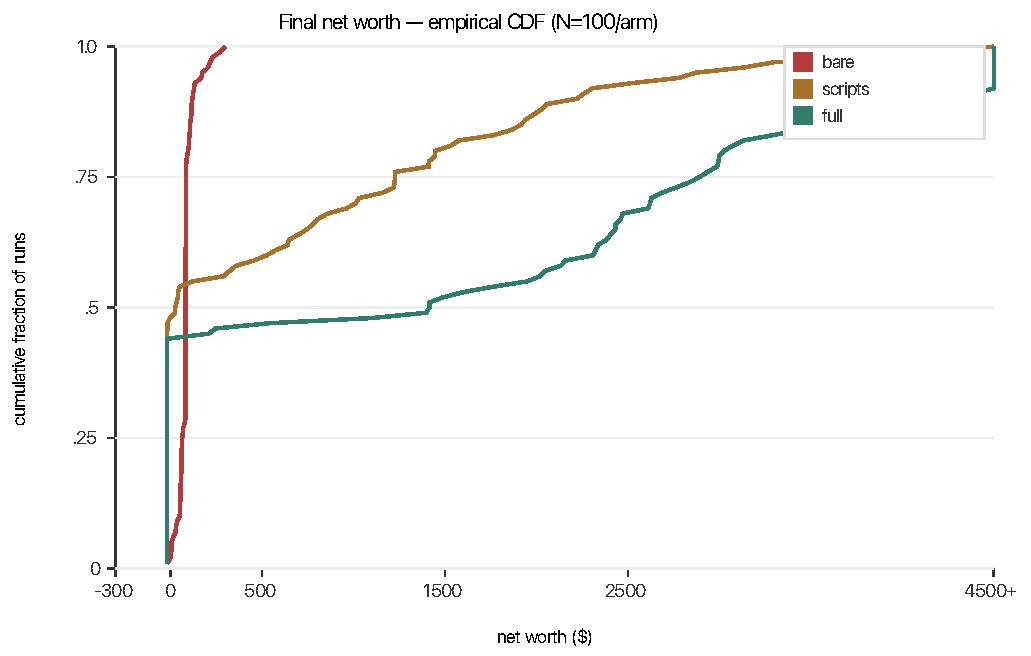
\includegraphics[width=0.82\linewidth]{fig1_ecdf.pdf}
\caption{Empirical CDF of final net worth by arm ($N=100$/arm).}
\label{fig:ecdf}
\end{figure}

Paired comparisons (matched seeds, $N=100$):

\begin{table}[h]
\centering
\small
\begin{tabular}{lccccc}
\toprule
comparison & mean $\Delta$/seed & median $\Delta$ & bootstrap 95\% CI & Wilcoxon $p$ & McNemar (comp.) \\
\midrule
full $-$ bare    & $+\$1,639$ & $+\$1,364$ & $[\$1,259,\ \$2,041]$ & $1.6\times10^{-7}$ & 54/0 \\
scripts $-$ bare & $+\$649$   & $-\$38$    & $[\$438,\ \$883]$     & $6.8\times10^{-4}$ & 41/0 \\
full $-$ scripts & $+\$990$   & $+\$386$   & $[\$740,\ \$1,247]$   & $1.3\times10^{-9}$ & 16/3 \\
\bottomrule
\end{tabular}
\end{table}

Full achieves substantially higher net worth than both baselines. Note the
scripts$-$bare \textbf{median} difference is negative ($-\$38$) despite a
positive mean: the scripted policy beats the naive baseline through its
winners, not at the median.

\subsection{The advantage grows with the success threshold (RQ4)}

Decomposing outcomes for full vs scripts (paired, $N=100$):

\begin{table}[h]
\centering
\small
\begin{tabular}{lccl}
\toprule
outcome (full vs scripts) & full & scripts & paired effect \\
\midrule
bankruptcy (terminated)   & 44\% & 47\% & risk diff $-3$~pp, 95\% CI $[-11,+5]$; McNemar $p=0.61$ \\
composite failure ($<\$500$) & 46\% & 59\% & risk diff $-13$~pp, 95\% CI $[-21,-5]$; McNemar $p=0.0044$ \\
net worth $\mid$ both survived & --- & --- & $+\$1,751$/seed, Wilcoxon $p=5\times10^{-9}$ \\
\bottomrule
\end{tabular}
\end{table}

We find \textbf{little evidence of a bankruptcy reduction} relative to the
scripted policy: the estimated difference is only 3 percentage points and its
confidence interval spans zero ($[-11,+5]$~pp), so the experiment does not
distinguish the two bankruptcy rates. This is \emph{not} evidence that the
rates are equal --- only that any difference is small and imprecisely
estimated. The harness's clear advantage is elsewhere: surviving businesses are
far more valuable, and the composite-failure rate is separated with a risk
difference whose CI excludes zero.

A dead/broke/thriving transition table (rows = each seed's outcome under
scripts, columns = its outcome under full, so cells count seeds) shows where
the 100 seeds actually move (Figure~\ref{fig:transition} renders the same
matrix as a heatmap --- green for improved, red for regressed, grey for
unchanged):

\begin{table}[h]
\centering
\begin{tabular}{lcccc}
\toprule
scripts $\downarrow$ / full $\rightarrow$ & dead & broke & thriving & (row total) \\
\midrule
\textbf{dead}     & 38 & 1 & 8  & 47 \\
\textbf{broke}    & 3  & 1 & 8  & 12 \\
\textbf{thriving} & 3  & 0 & 38 & 41 \\
\midrule
\textbf{(col total)} & 44 & 2 & 54 & 100 \\
\bottomrule
\end{tabular}
\end{table}

Two things are visible that aggregate rates hide. First, the harness nearly
empties the alive-but-broke middle (2 seeds under full vs 12 under scripts) and
lifts most of it to thriving. Second, the movement is not one-directional: 8
seeds that die under scripts thrive under full, but 3 seeds that thrive under
scripts die under full --- the harness is not a strict Pareto improvement on
survival, and the net shift toward thriving ($41\to54$) is what the paired
net-worth tests capture. (bare thrives on 0 seeds; it is omitted from the
table.)

\begin{figure}[h]
\centering
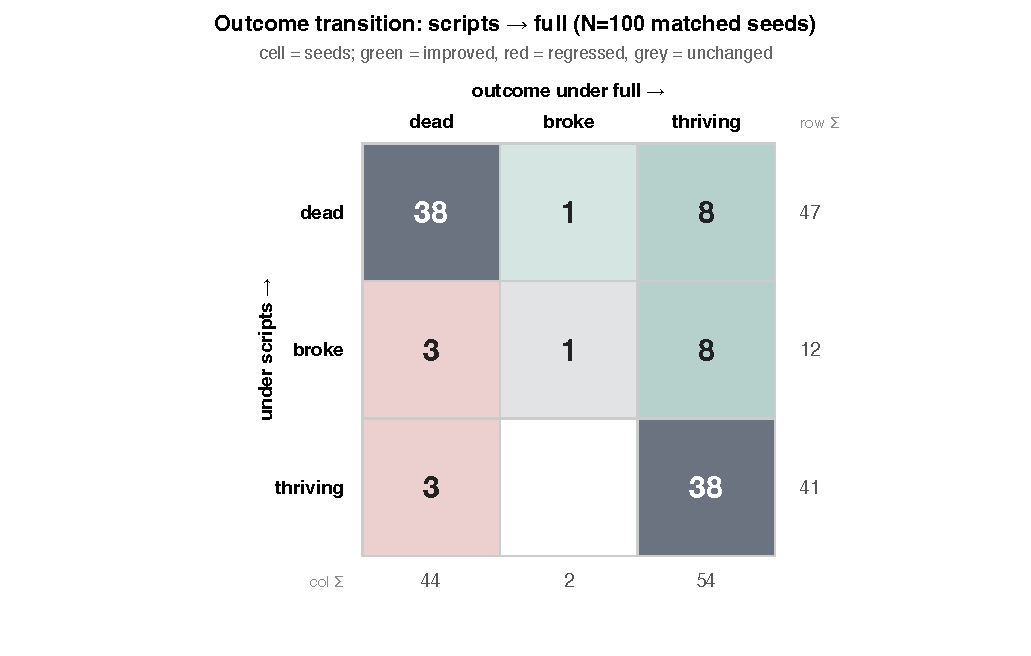
\includegraphics[width=0.7\linewidth]{fig7_transition.pdf}
\caption{Outcome transition scripts $\to$ full ($N=100$ matched seeds). Green =
improved, red = regressed, grey = unchanged; cell counts are seeds.}
\label{fig:transition}
\end{figure}

Threshold sensitivity shows the same story as an effect size: the
full-vs-scripts \emph{advantage} (scripts failure rate minus full failure rate)
grows as the success bar rises, with bootstrap CIs excluding zero from the
\$250 bar upward (Figure~\ref{fig:threshold}):

\begin{table}[h]
\centering
\begin{tabular}{lcccc}
\toprule
success bar & scripts fail\% & full fail\% & full advantage (pp) & 95\% CI \\
\midrule
terminated only & 47 & 44 & $+3$  & $[-5,+11]$ \\
$<\$250$        & 55 & 46 & $+9$  & $[+1,+17]$ \\
$<\$500$        & 59 & 46 & $+13$ & $[+5,+21]$ \\
$<\$1,000$      & 69 & 47 & $+22$ & $[+13,+31]$ \\
$<\$2,000$      & 87 & 55 & $+32$ & $[+23,+42]$ \\
\bottomrule
\end{tabular}
\end{table}

The advantage of the full harness over the scripted policy therefore increases
from 3~pp at the bankruptcy bar (indistinguishable from zero) to 32~pp at a
\$2,000 threshold --- the harness does not primarily keep the business alive; it
raises how much the survivors are worth.

\begin{figure}[h]
\centering
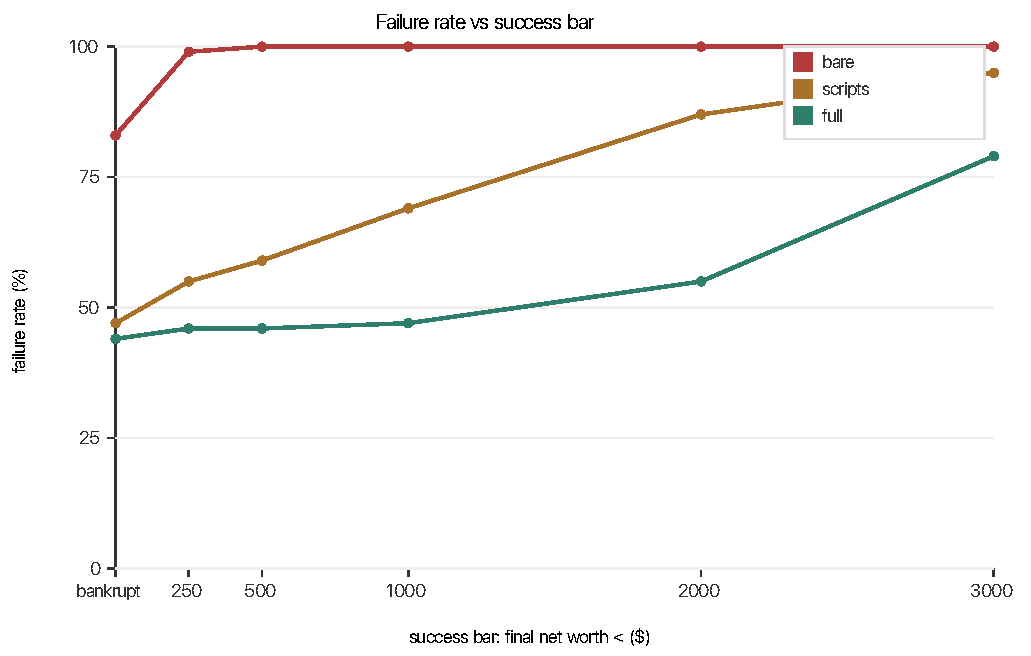
\includegraphics[width=0.82\linewidth]{fig2_threshold.pdf}
\caption{Failure rate vs.\ success bar, by arm. The full-vs-scripts gap widens
as the bar rises.}
\label{fig:threshold}
\end{figure}

\subsection{Mechanism: realized selling price, not throughput (RQ2); and how
bare fails}

\paragraph{The model's channel is price, not throughput.} To compare behavior
over an equal exposure window, we descriptively condition on the 47 seeds where
both policies reach day 200 and examine the back half of the run (days
101--200), per seed. This removes differential exposure time but conditions on
a post-treatment subset (survival is itself affected by the policy), so this
analysis is mechanistic/descriptive rather than a full-sample causal effect:

\begin{table}[h]
\centering
\begin{tabular}{lccc}
\toprule
metric (co-survivors, days 101--200) & scripts & full & paired $\Delta$ (full$-$scripts), 95\% CI \\
\midrule
units sold / day       & 52.6   & 51.7   & $-1.0\ [-3.0,+1.3]$ \\
realized price / unit  & \$1.57 & \$1.84 & $+\$0.27\ [+\$0.23,+\$0.32]$ \\
revenue / day          & \$83.1 & \$94.8 & $+\$11.7\ [+\$8.3,+\$15.5]$ \\
\bottomrule
\end{tabular}
\end{table}

The quantities reconcile per seed as an exact identity (price $\times$ volume =
revenue). There is \textbf{no evidence of a volume increase} under full --- the
estimated difference is $-1.0$ unit/day, with the 95\% interval ranging from
$-3.0$ to $+1.3$ (roughly $-5.7\%$ to $+2.5\%$ of the $\sim$52 units/day base)
--- whereas realized selling price rises by \textbf{\$0.27/unit ($\sim$17\%),
with the entire interval positive}. A per-seed symmetric (Shapley)
decomposition of the revenue difference into a price component $\Delta p \cdot
\bar q$ and a volume component $\Delta q \cdot \bar p$ makes the asymmetry
precise: the \textbf{price effect is $+\$13.75$/day $[+11.66,+15.99]$} while the
\textbf{volume effect is $-\$2.01$/day $[-5.33,+1.65]$}, and the two sum exactly
to the observed $+\$11.7$/day revenue gain. So the price effect is large enough
to \emph{more than} explain the revenue gain; the slight volume decline
partially offsets it.

Realized selling price is directly measured (revenue $\div$ units); we report
it rather than ``margin'' deliberately, because the procurement-cost tables
(\texttt{orders}, \texttt{price\_book}, \texttt{quotes}) are empty in these
runs, so cost of goods sold per unit --- and hence gross margin --- is
\textbf{not} recoverable from the archived logs. The mechanism we can defend is
therefore \emph{higher realized selling price at comparable throughput};
whether the full contribution margin also rises depends on unlogged COGS. Both
arms face the same deterministic supplier environment, although their
procurement decisions may differ (procurement is one of the seats the harness
routes to the model, \S3), so we do not claim procurement cost is held constant
--- only that the selling-price lever is directly measured and the seat ablation
in \S5.4 isolates pricing causally. Figure~\ref{fig:traj} plots median net
worth over time; the price premium compounds into the net-worth separation seen
there.

\begin{figure}[h]
\centering
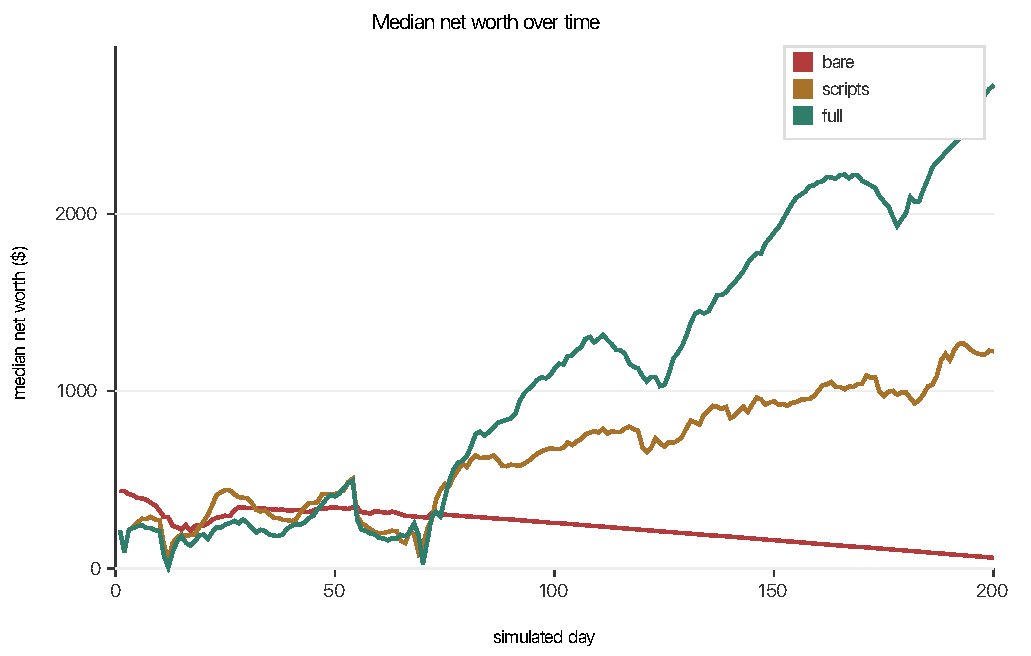
\includegraphics[width=0.82\linewidth]{fig3_trajectory.pdf}
\caption{Median net worth over time, by arm.}
\label{fig:traj}
\end{figure}

\paragraph{Bare's failure is immediate, not gradual.} Contrary to a ``loses the
thread over a long horizon'' reading, the bare arm sells $\sim$0.3 units/day
from the first week onward. It procures inventory and collects cash --- those
actions execute --- but never effectively prices or sells; net worth decays as
the fixed fee drains an inert business. Its $\sim$143-day median survival is
fee-arithmetic, not slow degradation. The failure is that the one-shot compound
decision is too much to juggle without scaffolding, and pricing is the dropped
sub-task. (Model outputs were unparseable on 7.7\% of bare days --- a minor
contributor; the other 92\% parse and still do not sell.)

\subsection{Component ablation: a strongly asymmetric result (RQ3)}

Removing harness components one at a time, matched-seed against full ($N=100$;
Figure~\ref{fig:diss}):

\begin{table}[h]
\centering
\begin{tabular}{lccc}
\toprule
arm & change from full & fail \% & median net worth \\
\midrule
full & --- (reference)             & 46  & \$1,415 \\
R1a  & gates removed               & 45  & \$1,378 \\
R1b  & persistent state removed    & 100 & $-\$18$ \\
\bottomrule
\end{tabular}
\end{table}

\begin{figure}[h]
\centering
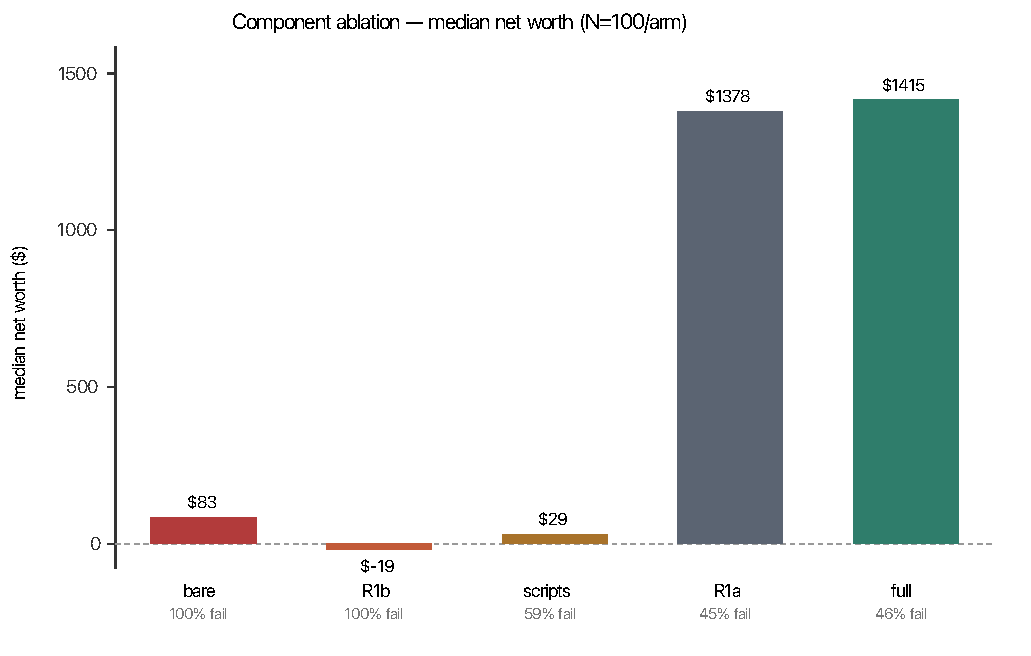
\includegraphics[width=0.82\linewidth]{fig4_dissociation.pdf}
\caption{Component ablation --- median net worth by arm ($N=100$/arm).}
\label{fig:diss}
\end{figure}

\paragraph{The gates are not necessary for median performance or failure
reduction under this workload.} Removing the entire gate suite leaves the
composite-failure rate essentially unchanged (45\% vs 46\%; paired risk
difference $-1$~pp, 95\% CI $[-11,+9]$; McNemar 13/12, $p=1.0$) and the paired
median net-worth difference at exactly \$0. The paired \emph{mean} net worth
actually rises when gates are removed ($+\$399$/seed), but this estimate is
imprecise and tail-driven: its bootstrap 95\% CI is $[-\$7,+\$822]$, which
includes zero, and the paired differences are wide, with a median of \$0 and
10th/90th percentiles of $-\$2,152$ / $+\$3,316$. The reading consistent with
all of this is that gates occasionally clip a below-floor move that would have
paid off in the right tail, while leaving the median run and the failure rate
unchanged; we do \textbf{not} claim the two arms are equivalent --- the CIs are
too wide for an equivalence verdict at any tight margin. Two facts help explain
why gate removal has little detectable effect on the median and failure rate in
this workload: gates bind on only 0.2\% of money actions in the full runs, and
the procurement/vendor subsystem they primarily protect is lightly exercised by
this simulator (\S7). (These contextualize the weak observed effect; they do
not bound the effect a rarely-binding gate could have in a workload that
stressed it --- a gate that fires on 0.01\% of actions could still avert a
catastrophic irreversible loss.) So the defensible statement is narrow:
\emph{under the proposal distribution this workload generates, the financial
gates were rarely causally active and their removal did not degrade median
performance or failure rate.} (Verified behaviorally: R1a's gates were
evaluated 403,441 times and denied none, versus 697 denials in full ---
enforcement is genuinely off; note the gate-config hash is identical across the
two, so the manifest hash does not capture whether enforcement is on, a
provenance gap flagged in \S7.)

\paragraph{Persistent structured state is necessary, and its removal is worse
than no harness.} Removing the state ledger collapses performance to 100\%
failure (98\% bankruptcy), median net worth $-\$18$ --- \emph{below} bare's
\$86. This is a genuine behavioral collapse, not a broken pipeline: R1b runs
lasted 183 days on average, made 511 model calls each, and traded $\sim$220
units per run. Because R1b retains the full specialized-call structure and
per-step budget, the comparison \textbf{rules out additional model calls or
task decomposition \emph{alone} as sufficient} to explain the full arm's
performance: the same call structure without persistent state produces
catastrophe. It does \textbf{not} show that decomposition contributes nothing
--- the two are plausibly complementary (decomposition helps only when state is
present; we lack the no-decomposition/with-state cell to separate them, since
bare differs in many other respects). What R1b establishes is the necessity of
the state treatment. We interpret this as the harness supplying persistent
structured state the weak model cannot hold in-context, but the treatment
bundles persistence, a canonical denoised representation, and fresh-prompt
context management, and this experiment does not isolate which of those is the
operative mechanism (\S7). That R1b underperforms bare is mechanistically
informative --- the harness's action structure, deprived of state to coordinate
it, drives the model to keep procuring and pricing incoherently, trading itself
into deeper insolvency than the near-inert baseline.

Together these give a strongly \textbf{asymmetric ablation}: removing
persistent structured state is catastrophic, while removing the gates is not
detectable at the median or on the failure rate. (We avoid the term ``double
dissociation'': that requires two components with selective effects on two
\emph{different} outcomes, which we do not demonstrate.)

\paragraph{Within a functioning harness, the pricing seat is necessary for ---
and appears to account for most of --- the model's advantage over the scripted
policy.} The harness routes several decisions to the model (pricing,
procurement, cash collection). Replacing only the pricing seat with a
deterministic rule (R5, $N=100$, matched seeds) \textbf{erases the full arm's
advantage} (Figure~\ref{fig:seat}): mean net worth falls to \$577 (scripts
\$735; full \$1,725) and the composite-failure rate rises to 65\%. Against full
the effect is decisive --- paired composite-failure McNemar 2/21 ($p<0.001$),
and surviving businesses worth roughly half as much (co-survivor mean \$1,714 vs
\$3,566; ratio 0.48). The mean gap has two components --- R5 produces both fewer
winners (35 vs 54) and smaller ones (winner-mean \$1,658 vs \$3,201) --- with the
size effect the larger of the two.

Against the scripted baseline, R5 does not merely match it --- it is
\emph{statistically indistinguishable on composite failure} (McNemar $p=0.27$)
and \emph{modestly worse on mean net worth} (R5$-$scripts $-\$158$, 95\% CI
$[-\$258,-\$75]$, median $-\$0$). This is more informative than ``R5 sits at the
scripted level'': conditional on scripted pricing, retaining the model's other
seats (procurement, cash collection) does not improve on the fully scripted
policy and is associated with slightly lower mean net worth. We cannot
additively attribute $-\$158$ to those seats --- interactions preclude that ---
but the finding indicates the model's value in this harness is \textbf{highly
localized}: pricing judgment more than compensates for whatever costs the
remaining model-mediated decisions impose, rather than the model being
generically useful throughout. We therefore identify pricing as a
\emph{necessary} model-mediated contributor while stopping short of ``pricing
carries the model's entire contribution'': establishing that the other seats
contribute nothing (or that a single seat carries everything) requires the
remaining per-seat ablations, which we have not run (\S7).

\begin{figure}[h]
\centering
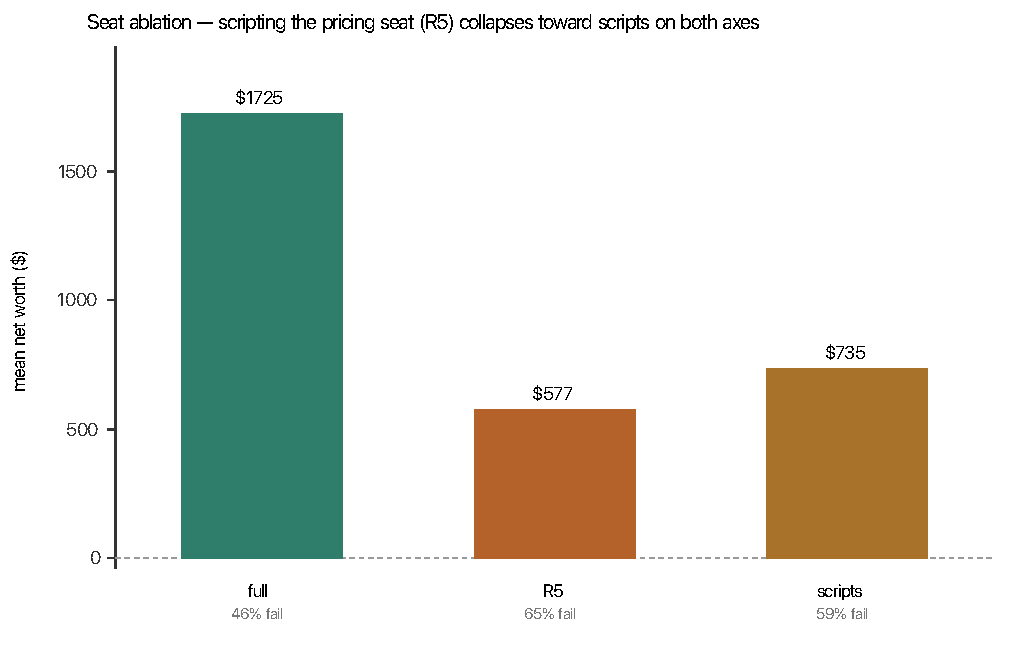
\includegraphics[width=0.82\linewidth]{fig5_seat.pdf}
\caption{Seat ablation: scripting the pricing seat (R5) erases the full arm's
advantage over the scripted baseline.}
\label{fig:seat}
\end{figure}

The mechanism we can defend is unified in direction: pricing sets the realized
selling price, increasing revenue per unit sold and potentially enlarging the
cash buffer available to absorb the environment's shocks; the archived logs do
not permit a direct gross-margin decomposition (COGS is unlogged, \S5.3).
Scripting the pricing seat removes that lever --- the causal complement to
\S5.3's realized-price finding, and convergent with the bare arm, whose fatal
omission was also pricing.

A further caveat scopes even the pricing result. R5 shows the model's pricing
policy beats \emph{this} deterministic pricing rule, which was written as
operational ``fundamentals,'' not tuned for optimality. It does not establish
that no simple model-free rule (e.g., an elasticity-aware or tuned-markup policy
given the same state) could recover the same value. Distinguishing ``the model
contributes flexible judgment'' from ``our baseline rule leaves obvious pricing
value on the table'' requires a stronger non-LLM pricing baseline, which we flag
as future work (\S7).

\section{Exploratory Studies}

The primary study is the three-arm comparison and the component ablation above.
We ran three further studies --- a capability gradient across model tiers, a
live-LLM adversary, and a durability push to a long horizon --- but each is
underpowered or off the primary simulator configuration, so we report them as
preliminary observations in \textbf{Appendix~B} rather than as results, to keep
them from lending unearned weight to the main claims. They motivate future work
(notably the multi-model full-arm curve); none is load-bearing for RQ1--RQ4.

\section{Threats to Validity}

\begin{itemize}
\item \textbf{Seed holdout and pre-specification.} The $N=100$ primary seeds
were not a held-out test set: the harness, scripts, prompts, thresholds, and
outcome definitions were fixed during development that inspected earlier smaller
batches and simulator instances, and $N=100$ was a round target, not a powered
one (\S4). As stated in the \S4 estimand, our intervals quantify variation over
the simulator's procedural environment distribution conditional on the
evaluated (development-tuned) implementation; because the seeds were not held
out, they are not an unbiased estimate of performance on untouched evaluation
instances. \textbf{The single strongest remaining validity step is a clean
held-out replication} --- a development seed set, a fresh untouched test seed
set, frozen code and prompts, and one final evaluation --- which we have not yet
run.
\item \textbf{Decoding stochasticity is not paired.} The design pairs the
\emph{simulator} condition on seed, but historical runs did not record a
decoding seed, so the model's stochastic realization is not matched across arms.
This is a sensible blocked design over environment seeds, but it means
``isolating the decision layer as the only variable'' is too strong:
environment-seed variance and LLM-sampling variance are not separated. A clean
replication should use deterministic decoding or record decoder seeds, ideally
with repeated decoding replicates on a subset of environment seeds to estimate
sampling variance directly.
\item \textbf{The state ablation is a bundle, not a single mechanism.} R1b
removes persistence, a canonical denoised state representation, and fresh-prompt
context management together. It establishes the necessity of the state
\emph{treatment}, not that persistence per se (rather than, say, a denoised
current-state brief) is the operative mechanism. Finer ablations --- persistent
ledger with a raw vs.\ canonical representation, a ledger with a growing vs.\
fresh transcript, current-operational-state vs.\ historical/vendor memory only
--- and a direct measurement of \textbf{state-reconstruction error} in R1b
(asking the model what it believes inventory, cost basis, and prices are, and
comparing to ground truth over the horizon) would turn the working-memory
interpretation into an observed mechanism. These are not attempted here.
\item \textbf{The gates are lightly stressed by this workload.} Gates bind on
only 0.2\% of money actions and the procurement/vendor subsystem is lightly
exercised, so the ``gates not necessary'' finding is scoped to \emph{this
proposal distribution} and does not establish that guardrails are unimportant
to agent performance in general. A targeted experiment constructed to contain
high-risk situations where gates actually bind is needed to evaluate their
value where it would matter.
\item \textbf{The pricing localization is one seat, not a full attribution.}
R5 establishes pricing as necessary, but interactions could mask contributions
from the other model seats (procurement, cash collection). The remaining
per-seat ablations (script each other seat individually) are required before
claiming pricing is the model's \emph{only} contribution.
\item \textbf{The pricing baseline is ``fundamentals,'' not optimized.} R5
compares the model against a deliberately simple deterministic pricing rule. A
stronger model-free pricing baseline (elasticity-aware, tuned markup, or a small
search) is needed to distinguish ``the model contributes flexible judgment''
from ``the baseline rule leaves obvious value on the table.''
\item \textbf{Co-survivor analysis is on a post-treatment subset.} The
$+\$1,751$/seed ``quality of survival'' figure conditions on seeds where
\emph{both} arms survived, and survival is itself affected by the policy; it
should be read as a description of the both-survived subset, not as a clean
causal decomposition. The threshold sweep and the full-sample net-worth
comparison (\S5.1--5.2) carry the broader claim.
\item \textbf{Single model in the primary arms.} The primary result shows a
scaffold rescues a \emph{weak} model; it does not show performance is
independent of capability. The multi-model full-arm curve is the pending test.
\item \textbf{No self-scaffolding control.} We tested ``the model cannot hold
state when we withhold it,'' not ``the model could not build state if given
tools.'' A tool-enabled model permitted to construct and maintain its own
scaffold is the fair capability ceiling and was not run.
\item \textbf{Bare is a control, not a capability verdict.} ``Unaided fails''
is not ``incapable.''
\item \textbf{Long-horizon framing.} The paper's framing invokes long-horizon
coherence, but bare fails essentially from the first week (\S5.3) --- its
failure is an immediate compound-decision/pricing omission, not gradual drift.
R1b is the arm that could substantiate a specifically long-horizon-memory
mechanism, but only if its state errors are shown to \emph{accumulate with
horizon}; we have not yet produced that evidence (e.g., state-reconstruction
error vs.\ day, or the full-vs-baseline advantage at 10/25/50/100/200-day
horizons). As it stands the paper establishes a scaffolding result on a
long-horizon task more firmly than it establishes a long-horizon-memory
\emph{mechanism}.
\item \textbf{Provenance gaps.} A simulator-config hash alone proved
insufficient earlier in the project (a code-level \texttt{placeOrder} fix left
same-hash runs incomparable), motivating full implementation provenance (git
commit, binary hash, quantization, decoding seed, prompt-template hashes). The
shared \texttt{sim\_config\_sha} (\texttt{64fa1ff5}) supports \emph{configuration}
consistency across arms but, absent a populated code commit, cannot by itself
prove the compiled implementation was identical. A concrete symptom: R1a carries
the same \emph{gate-config} hash as full despite gate enforcement being disabled
--- the manifest hash does not capture whether enforcement is on, which the
provenance schema should fix. Historical runs also lack recorded decoding seeds.
``Recomputable to the cent from archived databases'' is the accurate
reproducibility claim; rerunning stochastic model calls reproduces effect sizes,
not exact dollars. The cleanest remedy is to rerun the core arms with git commit
and decoder seed recorded.
\item \textbf{A negative result we retain.} A prototyped fix to the harness's
tendency to starve rather than overpay a predatory vendor appeared to add
survivors at $N=48$ but evaporated at $N=136$ ($-\$208$/seed); the starvation is
a deliberate net-worth-maximizing policy, not a bug. (The $N=136$ databases were
lost to infrastructure failure; this figure is from notes.)
\item \textbf{Ablation scope.} The ablation isolates state vs gates; finer
decomposition of \emph{which} state (inventory vs cost vs vendor memory) is not
attempted, and the procurement/vendor subsystem is lightly exercised in this
simulator.
\end{itemize}

\section{Discussion}

The result reframes what the harness is doing, within the scope this workload
supports. Under this proposal distribution it is not primarily a guardrail
system: the gates almost never bind, and removing them leaves the median run and
the failure rate unchanged. Its load-bearing component is persistent structured
state: the 4-billion-parameter model does not perform reliably when required to
operate without the harness's persistent structured-state treatment, and pricing
is a necessary model-mediated contribution on top of that substrate --- it sets
the realized selling price. We read the state result as the harness supplying
persistent structured state the weak model cannot hold in-context; we are
deliberately cautious about the stronger cognitive claim that this is
specifically the model's ``working memory,'' because the state treatment also
supplies a canonical denoised representation and fresh-prompt context
management, and this experiment does not separate persistence from
representation (\S7). The complementarity is nonetheless asymmetric: without the
state treatment, the resulting harness configuration performs even worse than
bare (R1b $<$ bare), consistent with an action-taking architecture amplifying
incoherent decisions when its coordinating state is removed.

The seat ablation carries a further engineering implication worth stating, if
not overselling. Full (model pricing + other model seats) beats scripts by
$+\$990$/seed, whereas R5 (scripted pricing + the same other model seats) is
\$158/seed \emph{below} scripts: one model-mediated decision appears valuable
enough to more than overcome the aggregate cost of leaving the remaining
decisions with the weak model. We cannot decompose that aggregate cost
(interactions preclude it, \S5.4), but the pattern suggests a design heuristic
beyond this simulator: hybrid systems may gain more from selectively allocating
model judgment to the few decisions with high upside than from maximizing the
number of decisions delegated to the model. We offer this as a hypothesis
motivated by one seat ablation, not a demonstrated general law.

\paragraph{A design corollary, illustrated by the study's own process.}
Conducting this study was itself a long-horizon process executed partly by
agents, and it failed twice at exactly the steps left to an agent's judgment
rather than a gate: an ungated teardown destroyed a set of runs by skipping a
sync step, and a silently mis-parsed configuration flag corrupted a comparison
for days (surfaced only because the manifest hashes the simulator config). Both
are instances of the same design principle the harness embodies --- externalize
the state, gate the irreversible step, verify before an action becomes
irreversible --- and both are anecdotes about process discipline, not controlled
evidence. We include them as motivation, not as a second demonstration of a
general law; the relationship between a model losing state and an experimenter
skipping a gate is an analogy across different mechanisms, not identical
causation.

\section{Conclusion}

On a long-horizon business simulator with adversarial supplier profiles, a
scaffolding harness moves a weak 4B model from 100\% composite failure (median
net worth \$83) to 54\% success (median \$1,415), and within the harness that
performance depends on the persistent structured-state treatment: neither gate
enforcement nor the additional model calls and task decomposition alone explains
the observed advantage. Removing the state substrate collapses the arm to total
failure, while removing the gates does not measurably degrade median net worth
or failure rate. The harness does not measurably keep the model \emph{solvent}
relative to a scripted policy (bankruptcy differs by 3~pp, CI spanning zero);
its clear advantage grows with the success threshold, and pricing is necessary
for that observed advantage. A seat-level ablation shows this: scripting the
pricing seat alone erases the full arm's advantage --- the result is
statistically indistinguishable from the deterministic policy on composite
failure and modestly \emph{worse} on mean net worth --- identifying pricing as a
necessary model-mediated contributor, and indicating that the model's value in
this harness is highly localized rather than distributed across its decisions.
We deliberately hold the claims narrow --- necessity under this workload, not a
general law --- and the strongest open tests remain for future work: a held-out
replication with recorded decoding seeds, the remaining per-seat ablations, a
stronger model-free pricing baseline, and a tool-enabled model permitted to
build its own scaffold.

\appendix

\section{Reproducibility}

Archived run databases and analysis scripts are in the accompanying
reproducibility package. \texttt{compute\_results.py} regenerates the core
three-arm, paired, capability-gradient, and exploratory numbers;
\texttt{phase1\_stats.py} the quantiles, bootstrap CIs, Wilcoxon tests,
separated failure tests, and threshold sweep; \texttt{phase1\_mechanism.py} the
trajectory and efficiency analyses; \texttt{phase1\_gates\_bare.py} the
gate-rejection rates and bare-behavior breakdown; \texttt{verify\_r1.py} the
R1a/R1b ablation paired comparisons and the R1b real-vs-artifact check;
\texttt{verify\_r5.py} the R5 seat-ablation paired comparisons (vs full and vs
scripts); \texttt{verify\_revision.py} the R1a full paired statistics
(mean/median difference, bootstrap CI, quantiles, composite-failure risk
difference), the scripts$\to$full dead/broke/thriving transition table, the
bankruptcy and threshold-sweep risk differences with CIs, the co-survivor
realized-price/volume/revenue table, the per-seed Shapley price-vs-volume
revenue decomposition, and the R5-vs-scripts net-worth paired test;
\texttt{figures.py} regenerates all seven figures as dependency-free SVG.
Failure is defined as termination or final net worth below \$500. All
comparisons are matched-seed. The primary three arms share simulator-config
hash \texttt{64fa1ff5}.

\section{Preliminary Observations (underpowered; not part of the main result)}

These are stress tests, not powered experiments, and each is either underpowered
or off the primary simulator configuration. We report them to motivate future
work; none supports the main claims (RQ1--RQ4).

\paragraph{Capability gradient (bare arm, across model tiers).} Bare-arm net
worth rises with model tier --- \texttt{gemma3:4b} \$86 (100\% fail),
\texttt{qwen2.5:7b} \$171 (100\% fail), \texttt{deepseek-v4-flash} \$2,452 (50\%
fail) --- suggesting the harness's necessity is greatest for the weakest models
(Figure~\ref{fig:cap}). This does \textbf{not} establish model-independence of
the full arm, which requires the (unrun) multi-model full-arm curve. This is the
one exploratory result we would carry forward, as it directly motivates the
pending multi-model study.

\begin{figure}[h]
\centering
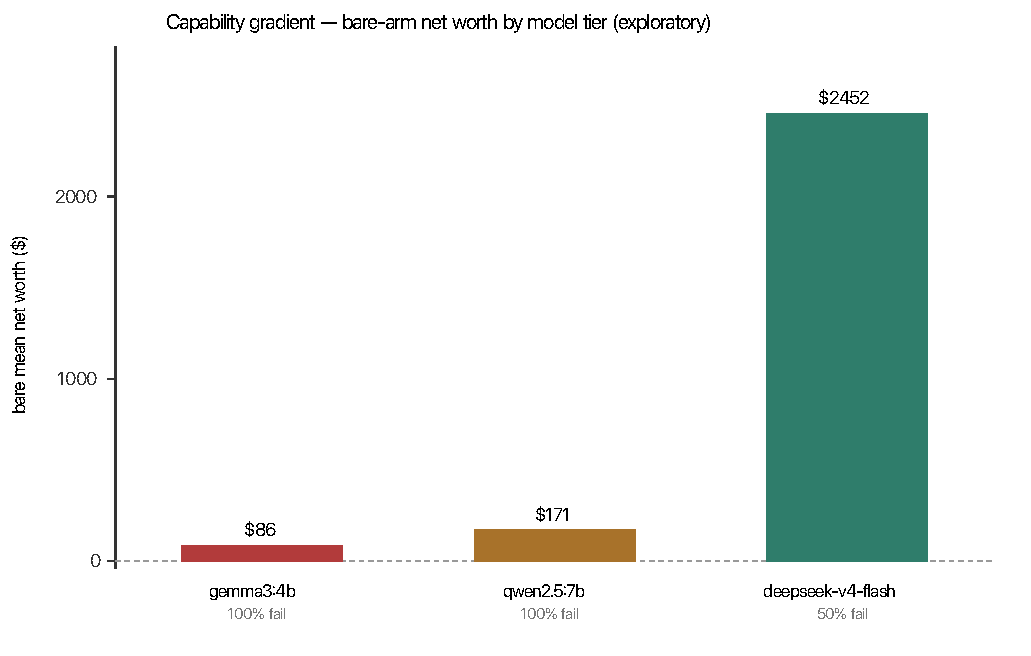
\includegraphics[width=0.82\linewidth]{fig6_capability.pdf}
\caption{Capability gradient --- bare-arm net worth by model tier (exploratory).}
\label{fig:cap}
\end{figure}

\paragraph{Harness on a capable model.} On \texttt{deepseek-v4-flash} (paired,
$n=10$), full beats bare on both net worth ($+\$3,607$/seed, $t=2.48$) and
failure rate (10\% vs 50\%), suggesting the harness helps even a stronger model.
Small $n$; directional only.

\paragraph{Live adversary.} Replacing scripted suppliers with a larger live
model (\texttt{qwen2.5:7b}) for supplier dialogue, $n=3$ selected seeds ran
577--985 days with zero bankruptcies. This shows long-horizon coherence against
live-LLM-mediated suppliers is \emph{achievable}; $n=3$ cannot establish a rate,
the sim config differs from the ablation, and whether the vendor model
controlled economically consequential behavior (versus dialogue only) is not
established.

\paragraph{Durability.} Five near-median seeds pushed toward a 3,000-day cap:
two bankrupt early (on-distribution), three compounded with monotonically rising
net worth past day 365 before infrastructure loss. Demonstrates achievability of
500+ day coherence, not a survival rate; the seeds were selected and the
survivors are right-censored by infrastructure failure.

\begin{thebibliography}{99}

\bibitem{vendingbench} Backlund, A., \& Petersson, L. (2025).
\emph{Vending-Bench: A Benchmark for Long-Term Coherence of Autonomous Agents.}
arXiv:2502.15840. \url{https://arxiv.org/abs/2502.15840}

\bibitem{bmad} BMAD Code. \emph{BMAD-METHOD} (v6.x.x) [software]. GitHub.
\url{https://github.com/bmad-code-org/bmad-method}

\bibitem{anthropic} Anthropic. (2024). \emph{Building Effective Agents.}
Anthropic Engineering.
\url{https://www.anthropic.com/engineering/building-effective-agents}

\bibitem{gemma} Google. \emph{Gemma 3 Model Card.} Google AI for Developers.
\url{https://ai.google.dev/gemma/docs/core/model_card_3}

\bibitem{gaia} Mialon, G., Fourrier, C., Swift, C., Wolf, T., LeCun, Y., \&
Scialom, T. (2023). \emph{GAIA: A Benchmark for General AI Assistants.}
arXiv:2311.12983. \url{https://arxiv.org/abs/2311.12983}

\bibitem{taubench} Yao, S., Shinn, N., Razavi, P., \& Narasimhan, K. (2024).
\emph{$\tau$-bench: A Benchmark for Tool-Agent-User Interaction in Real-World
Domains.} arXiv:2406.12045. \url{https://arxiv.org/abs/2406.12045}

\bibitem{memgpt} Packer, C., Wooders, S., Lin, K., Fang, V., Patil, S. G.,
Stoica, I., \& Gonzalez, J. E. (2023). \emph{MemGPT: Towards LLMs as Operating
Systems.} arXiv:2310.08560. \url{https://arxiv.org/abs/2310.08560}

\bibitem{genagents} Park, J. S., O'Brien, J. C., Cai, C. J., Morris, M. R.,
Liang, P., \& Bernstein, M. S. (2023). \emph{Generative Agents: Interactive
Simulacra of Human Behavior.} arXiv:2304.03442.
\url{https://arxiv.org/abs/2304.03442}

\bibitem{voyager} Wang, G., Xie, Y., Jiang, Y., Mandlekar, A., Xiao, C., Zhu,
Y., Fan, L., \& Anandkumar, A. (2023). \emph{Voyager: An Open-Ended Embodied
Agent with Large Language Models.} arXiv:2305.16291.
\url{https://arxiv.org/abs/2305.16291}

\bibitem{coala} Sumers, T. R., Yao, S., Narasimhan, K., \& Griffiths, T. L.
(2023). \emph{Cognitive Architectures for Language Agents.} arXiv:2309.02427.
\url{https://arxiv.org/abs/2309.02427}

\bibitem{react} Yao, S., Zhao, J., Yu, D., Du, N., Shafran, I., Narasimhan, K.,
\& Cao, Y. (2022). \emph{ReAct: Synergizing Reasoning and Acting in Language
Models.} arXiv:2210.03629. \url{https://arxiv.org/abs/2210.03629}

\bibitem{reflexion} Shinn, N., Cassano, F., Berman, E., Gopinath, A.,
Narasimhan, K., \& Yao, S. (2023). \emph{Reflexion: Language Agents with Verbal
Reinforcement Learning.} arXiv:2303.11366.
\url{https://arxiv.org/abs/2303.11366}

\end{thebibliography}

\end{document}
